\documentclass[hyperref={unicode}, xcolor={svgnames, table},
usepdftitle=false]{beamer}

\usetheme{Boadilla}
\usecolortheme{beaver}
\usefonttheme{serif}
\setbeamercovered{dynamic}

\setbeamertemplate{enumerate items}[square]
\setbeamertemplate{section in toc}[square]
\setbeamertemplate{navigation symbols}{}

\usepackage[T2A]{fontenc}
\usepackage[utf8]{inputenc}

\usepackage[macedonian]{babel}
\usepackage[babel]{microtype}

\usepackage{mathtools, amssymb, amsthm, centernot}

\usepackage{graphicx, caption, subcaption}

\usepackage{booktabs, array, multicol}
\usepackage[newfloat]{minted}

\usepackage{csquotes}

\usepackage[os=win]{menukeys}
\usepackage{tikz}

\usepackage{siunitx}
\sisetup{%
  detect-all,
  round-mode=places,
  round-precision=2,
  group-separator=.,
  output-decimal-marker={,}
}

\deftranslation[to=macedonian]{Theorem}{Теорема}
\deftranslation[to=macedonian]{theorem}{теорема}
\deftranslation[to=macedonian]{Definition}{Дефиниција}
\deftranslation[to=macedonian]{definition}{дефиниција}

\DeclareMathOperator*{\argmax}{arg\,max}
\DeclareMathOperator*{\argmin}{arg\,min}
\DeclarePairedDelimiter\abs{\lvert}{\rvert}
\DeclarePairedDelimiter\norm{\lVert}{\rVert}

\newcommand\independent{\protect\mathpalette{\protect\independenT}{\perp}}
\def\independenT#1#2{\mathrel{\rlap{$#1#2$}\mkern2mu{#1#2}}}

\graphicspath{{Figures/}}

\hypersetup{%
  pdfinfo={%
    Title={Вовед во R},
    Subject={Статистика},
    Author={Дарио Ѓорѓевски},
    Keywords={Статистика, Тестирање на статистички хипотези, t-тест, F-тест,
      хи-квадрат тест, линеарна регресија}
  }
}

\theoremstyle{remark}
\newtheorem*{remark}{Забелешка}

\title{Вовед во R}

\subtitle{Тестирање на статистички хипотези и линеарна регресија}

\author[Дарио Ѓорѓевски]{%
  Дарио Ѓорѓевски\inst{1}\\%
  \href{mailto:gjorgjevski.dario@students.finki.ukim.mk}%
  {\texttt{gjorgjevski.dario@students.finki.ukim.mk}}
}

\institute[ФИНКИ]{%
  \inst{1}Факултет за компјутерски науки и инженерство\\%
  Универзитет Св.\ Кирил и Методиј, Скопје
}

\date{\today}

\logo{
\includegraphics[height=0.66cm]{Logo.png}}

\AtBeginSection[]{%
  \begin{frame}{Содржина}
    \tableofcontents[currentsection, hideothersubsections]
  \end{frame}
}

\begin{document}

\begin{frame}
  \titlepage
\end{frame}

\section{Распределби користени во статистиката}

\begin{frame}{\(\chi^2\)-распределба}{Дефиниција}
  \begin{definition}[\(\chi^2\)-распределба]
    Нека \(Z_1, \ldots, Z_{\nu}\) бидат независни и идентично распределени
    \(\mathcal{N}(0, 1)\) случајни променливи.  Тогаш,
    \[
      Q \coloneqq \sum\limits_{i = 1}^{\nu} Z_i^2
    \]
    има \(\chi^2\)-распределба со \(\nu\) степени на слобода,
    \[
      Q \sim \chi^2_{\nu}\text{.}
    \]
  \end{definition}
  \(\chi^2\)-распределбата е специјален случај на гама распределбата.  Сепак,
  иако тој резултат е од теориска значајност, во статистиката не е многу корисен.
\end{frame}

\begin{frame}{\(\chi^2\)-распределба}{pdf и CDF}
  Густината на \(\chi^2_{\nu}\)-распределбата е дадена со
  \[
    p(x; \nu) =
    \begin{cases}
      \frac{x^{\nu / {2} - 1} e^{-x / {2}}}{2^{\nu / {2}} \Gamma(\nu / {2})} & x
      > 0
      \\
      0 & \text{инаку.}
    \end{cases}
  \]
  \begin{figure}
    \centering
    \begin{subfigure}[b]{.475\linewidth}
      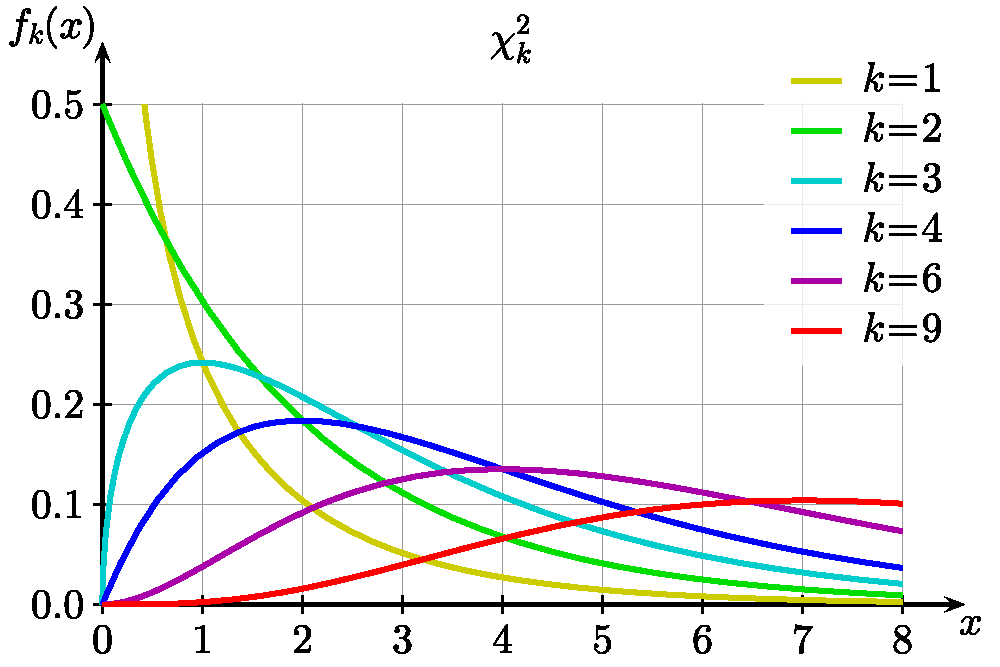
\includegraphics[width=\textwidth]{chi-square_pdf.pdf}
    \end{subfigure}
    \begin{subfigure}[b]{.475\linewidth}
      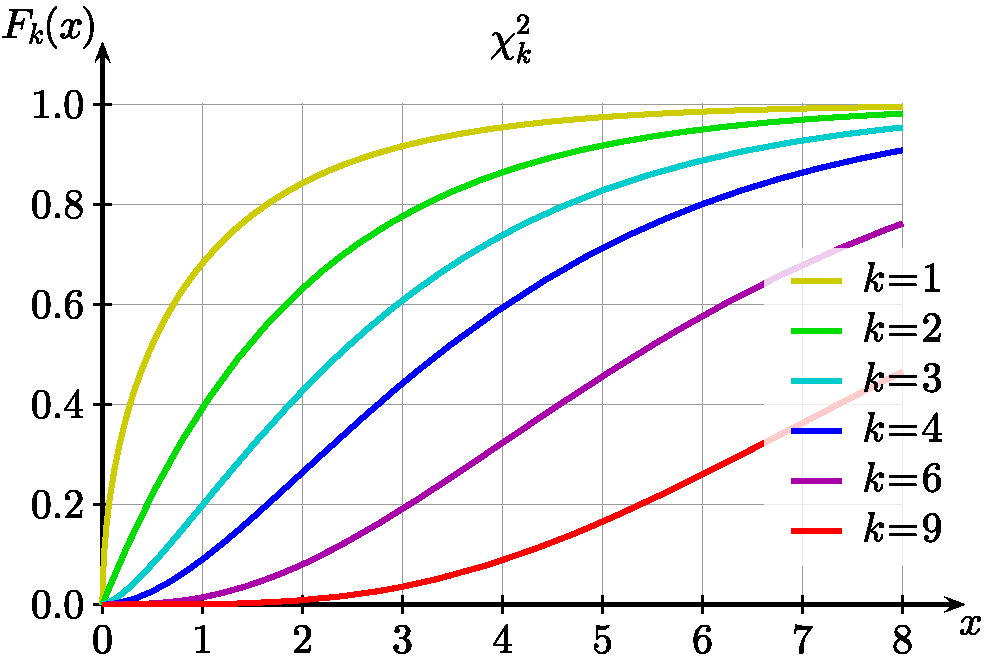
\includegraphics[width=\textwidth]{chi-square_CDF.pdf}
    \end{subfigure}
    \caption{Густина и функција на распределба за \(\chi^2_k\).}
  \end{figure}
\end{frame}

\begin{frame}{\(\chi^2\)-распределба}{Значајност во статистиката}
  Де Муавр и Лаплас имаат покажано дека биномната распределба може да биде
  апроксимирана со нормална, т.е.
  \[
    \chi \coloneqq \frac{m - N p}{\sqrt{N p q}} \xrightarrow{d} \mathcal{N}(0, 1)\text{,}
  \]
  каде \(m\) е бројот на успеси во \(N\) обиди, \(p\) е веројатноста за успех и
  \(q \coloneqq 1 - p\).  Ако ги кренеме двете страни на квадрат, добиваме
  \begin{equation}\label{eq:binomial-approximation}
    \chi^2 = \frac{(m - N p)^2}{N p q} = \frac{(m - N p)^2}{N p} + \frac{(N - m
      - N q)^2}{N q}\text{.}
  \end{equation}
\end{frame}

\begin{frame}{\(\chi^2\)-распределба}{Значајност во статистиката}
  Изразот даден со~\eqref{eq:binomial-approximation} ќе биде генрализиран од
  страна на Пирсон.
  \begin{theorem}[Пирсонов \(\chi^2\)-тест]
    Нека \(n\) биде број на категории, \(O_i\) број на набљудувања од категорија
    \(i\), а \(E_i = N p_i\) очекуван број набљудувања од категорија \(i\) даден
    од нултата хипотеза за \(p_i\).  Тогаш статистиката
    \[
      \chi^2 = \sum\limits_{i = 1}^{n} \frac{(O_i - E_i)^2}{E_i}
    \]
    има \(\chi^2\)-распределба со број на степени на слобода еднаков на бројот
    на оценети параметри.
  \end{theorem}
\end{frame}

\begin{frame}{\(\chi^2\)-распределба}{Значајност во статистиката}
  Друг значаен резултат ја поврзува \(\chi^2\) распределбата со распределбата на
  дисперзијата на примерок од нормлана распределба.
  \begin{theorem}[Својства на \(S^2\) за примерок од
    \(\mathcal{N}(\mu, \sigma^2)\) распределба]
    Нека \((X_1, X_2, \ldots, X_n)\) биде случаен примерок од обележје
    \(X \sim \mathcal{N}(\mu, \sigma^2)\).  Тогаш, \(\bar{X}\) и \(S^2\) се
    независни, и
    \[
      \frac{(n - 1) S^2}{\sigma^2} = \frac{\sum\nolimits_{i = 1}^{n} (X_i -
        \bar{X})^2}{\sigma^2} \sim \chi^2_{n - 1}\text{.}
    \]
  \end{theorem}
  Преку оваа теорема и \(F\)-распределбата, \(\chi^2\)-распределбата влегува во
  статистичките методи за анализа на дисперзија.
\end{frame}

\begin{frame}{\(t\)-распределба}{Дефиниција}
  \begin{definition}[\(t\)-распределба]
    Нека \(X_1, \ldots, X_n\) бидат независни и идентично распределени
    \(\mathcal{N}(\mu, \sigma^2)\) случајни променливи.  Тогаш, случајната
    променлива
    \[
      T = \frac{\bar{X} - \mu}{S / {\sqrt{n}}}
    \]
    има \(t\)-распределба со \(\nu = n - 1\) степени на слобода.
  \end{definition}
  Неформално, \(t\)-распределбата ја дава распределбата на \(\mu\) во однос на
  \(\bar{X}\), а поделено со стандардната девијација на примерокот и помножено
  со нормализирачка константа \(\sqrt{n}\).
\end{frame}

\begin{frame}{\(t\)-распределба}{Проширување на дефиницијата}
  Знаеме дека за примерок од нормална распределба,
  \begin{align*}
    (n - 1) \frac{S^2}{\sigma^2} &\eqqcolon V \sim \chi^2_{n - 1}\text{, и} \\
    (\bar{X} - \mu) \frac{\sqrt{n}}{\sigma} &\eqqcolon Z \sim \mathcal{N}(0, 1)\text{.}
  \end{align*}
  Така, запишеме ако \(\nu \coloneqq n - 1\),
  \[
    T \coloneqq \frac{Z}{\sqrt{V / {\nu}}} \sim t_{\nu} = \frac{\mathcal{N}(0,
      1)}{\sqrt{\chi^2_{\nu} / {\nu}}}\text{.}
  \]
  Во оваа форма \(t\)-распределбата се користи во тестови за просеци
  (\(t\)-тестови) како и во линеарната регресиона анализа.
\end{frame}

\begin{frame}{\(t\)-распределба}{pdf и CDF}
  Густината на \(t\)-распределбата со \(\nu\) степени на слобода е дадена со
  \[
    p(x; \nu) = \frac{\Gamma((\nu + 1) / {2})}{\sqrt{\nu \pi} \Gamma(\nu / {2})}
    \left(1 + \frac{x^2}{\nu}\right)^{- (\nu + 1) / {2}}\text{,}
  \]
  каде \(\Gamma(\cdot)\) е гама функцијата.
  \begin{figure}
    \centering
    \begin{subfigure}[b]{.45\linewidth}
      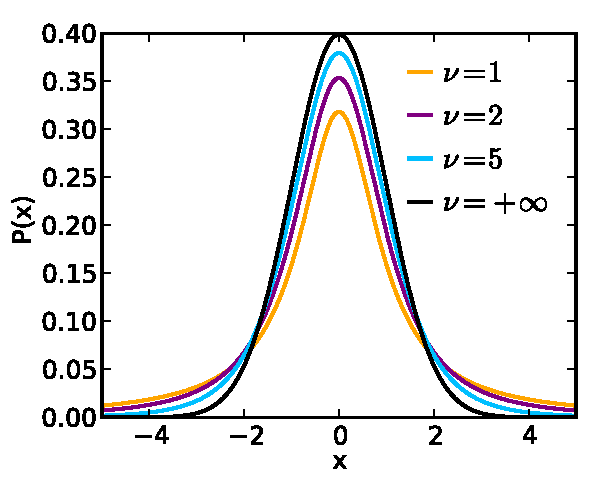
\includegraphics[width=\textwidth]{t_pdf.pdf}
    \end{subfigure}
    \begin{subfigure}[b]{.45\linewidth}
      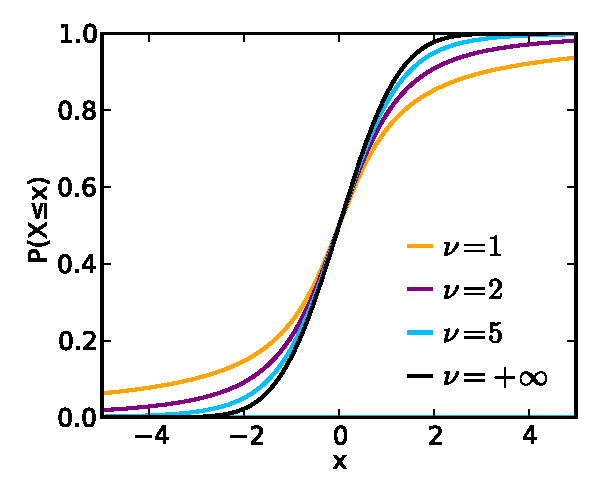
\includegraphics[width=\textwidth]{t_CDF.pdf}
    \end{subfigure}
    \caption{Густина и функција на распределба за \(t_{\nu}\).}
  \end{figure}
\end{frame}

\begin{frame}{\(F\)-распределба}{Дефиниција}
  \begin{definition}[\(F\)-распределба]
    \(F\)-распределбата се јавува како однос на две \(\chi^2\)-распределби
    склаирани со соодветните степени на слобода.  Имено, ако
    \(U_1 \sim \chi^2_{\nu_1}\), \(U_2 \sim \chi^2_{\nu_2}\), и
    \(U_1 \independent U_2\), тогаш
    \[
      X \coloneqq \frac{U_1 / {\nu_1}}{U_2 / {\nu_2}}
    \]
    има \(F\)-распределба со параметри (степени на слобода) \(\nu_1\) и
    \(\nu_2\).
  \end{definition}
\end{frame}

\begin{frame}{\(F\)-распределба}{pdf и CDF}
  Густината на \(F\)-распределбата со параметри \(\nu_1, \nu_2 > 0\) е дадена со
  \[
    f(x; \nu_1, \nu_2) = \frac{\sqrt{\frac{(\nu_1 x)^{\nu_1}
          \nu_2^{\nu_2}}{(\nu_1 x + \nu_2)^{\nu_1 + \nu_2}}}}{x
      \operatorname{B}(\nu_1 / {2}, \nu_2 / {2})}\text{,}
  \]
  каде \(\operatorname{B}(\cdot)\) е бета функцијата.
  \begin{figure}
    \centering
    \begin{subfigure}[b]{.45\linewidth}
      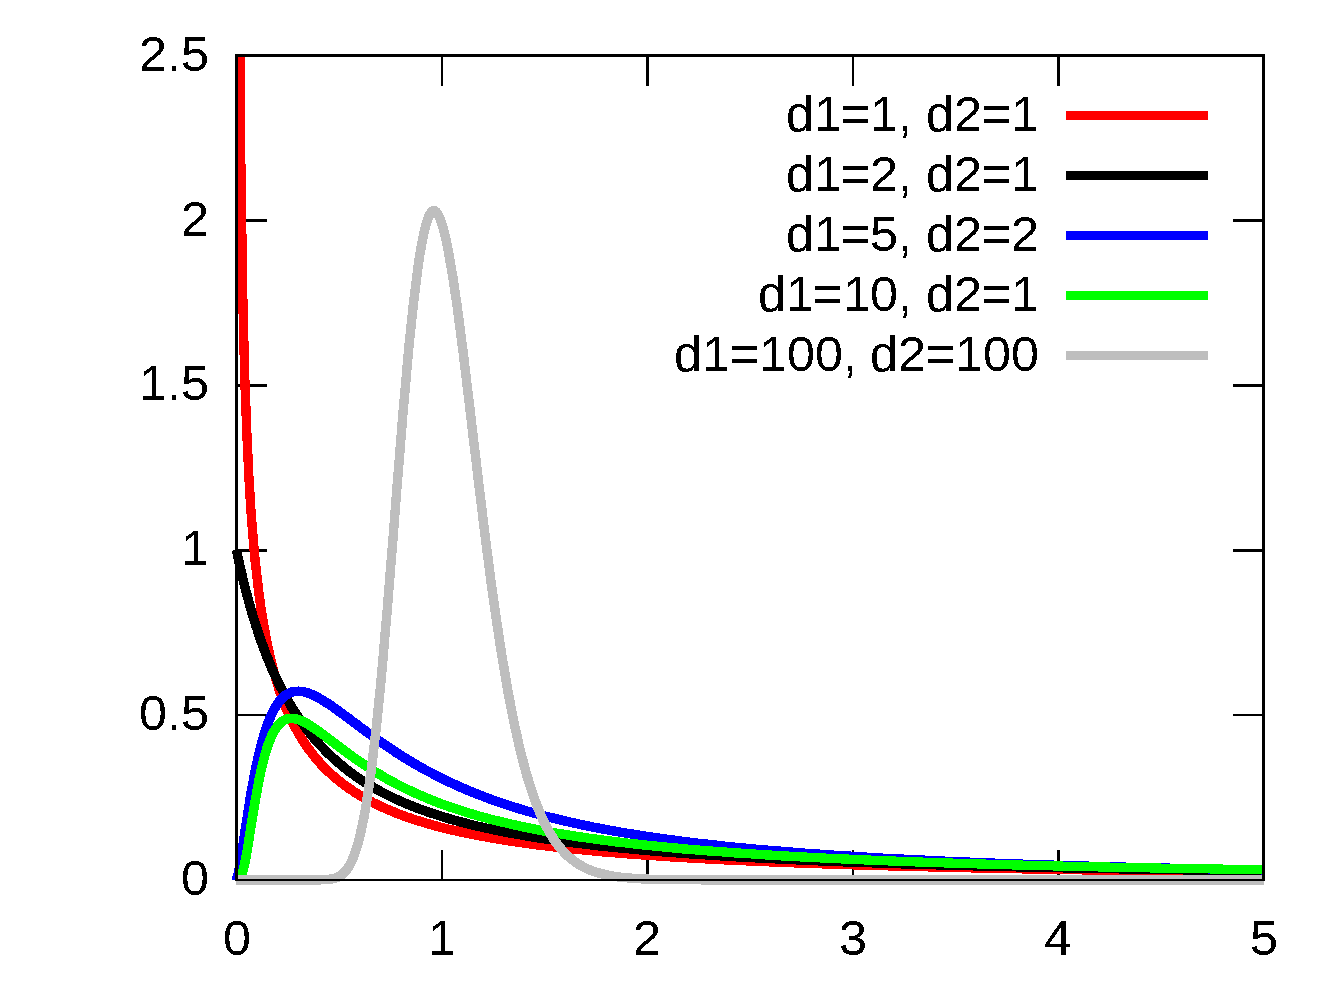
\includegraphics[width=\textwidth]{F_pdf.pdf}
    \end{subfigure}
    \begin{subfigure}[b]{.45\linewidth}
      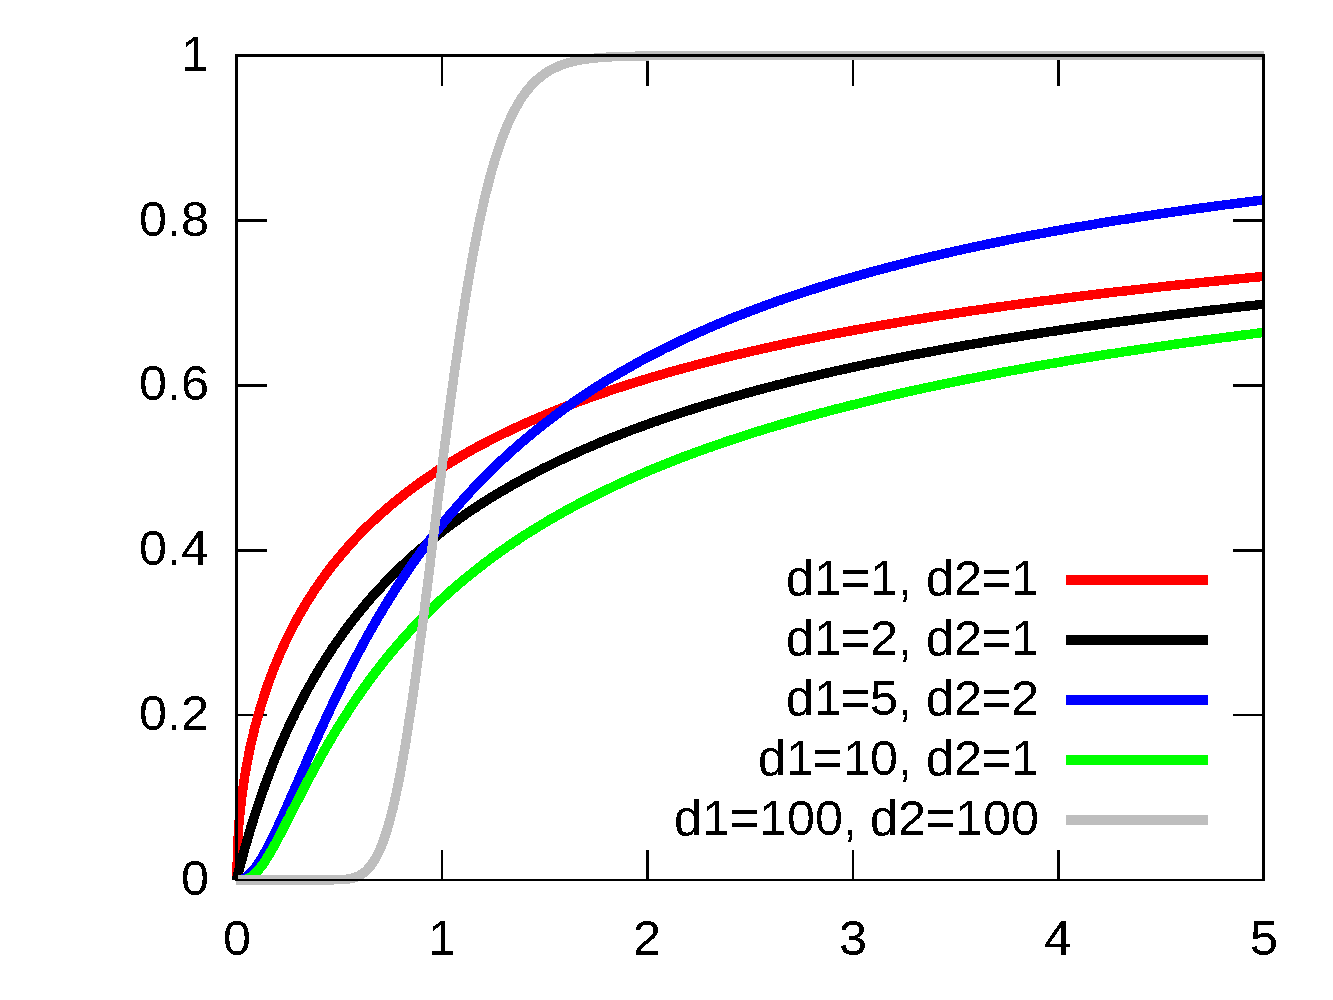
\includegraphics[width=\textwidth]{F_CDF.pdf}
    \end{subfigure}
    \caption{Густина и функција на распределба за \(F_{d_1, d_2}\).}
  \end{figure}
\end{frame}

\begin{frame}{\(F\)-распределба}{Значајност во статистиката}
  Видовме дека за примерок од нормална распределба,
  \(S^2 \sim \frac{\sigma^2 \chi^2_{n - 1}}{n - 1}\).  Така, ако имаме примероци
  со големини \(m\) и \(n\) од независни обележја
  \(X \sim \mathcal{N}(\mu_X, \sigma_X^2)\) и
  \(Y \sim \mathcal{N}(\mu_Y, \sigma_Y^2)\),
  \begin{equation}\label{eq:F-statistic}
    F \coloneqq \frac{S_X^2 / {\sigma_X^2}}{S_Y^2 / {\sigma_Y^2}} \sim F_{m - 1,
      n - 1}\text{.}
  \end{equation}
  Оваа статистика ни дава основа за анализа на еднаквост на дисперзија на
  примероци од нормално распределени обежеја.  Имено, ако нултата хипотеза е
  дека дисперзиите на двете обележја за еднакви, тогаш тие се кратат
  во~\eqref{eq:F-statistic}.
\end{frame}

\section{Тестирање на статистички хипотези}

\begin{frame}{\(t\)-тестови}{Вовед}
  \begin{itemize}
  \item \(t\)-тестови се тестови во кои тест статистиката има \(t\)-распределба
    под нултата хипотеза.
  \item Како што видовме, \(t\)-распределбата се јавува кога тест статистиката
    би имала нормална распределба доколку се знае вредноста на скалирачкиот
    параметар, обично \(\sigma^2\).
  \item Кога скалирачкиот параметар се замени со неговата вредност од
    примерокот, се добива \(t\)-распределена статистика.
  \item Благодарение на CLT, \(t\)-статистиките се особено поволни за тестови
    поврзани со просекот на едно обележје, односно разлика на просеци на две
    обележја.
  \end{itemize}
\end{frame}

\begin{frame}{\(t\)-тест за просек на обележје}{Дефиниција}
  \begin{itemize}
  \item Примерок \((X_1, \ldots, X_n)\) од обележје со просек \(\mu\).
  \item Нултата хипотеза е од облик \(\mu = \mu_0\), додека алтернативната е
    \(\mu \ne \mu_0\), \(\mu < \mu_0\), или \(\mu > \mu_0\).
  \item \(t\)-статистиката е од облик
    \[
      T = \frac{\bar{X} - \mu_0}{S / {\sqrt{n}}}\text{.}
    \]
    Оваа статистика има \(t_{n - 1}\) распределба кога
    \begin{itemize}
    \item примерокот доаѓа од нормално обележје; или
    \item примерокот е голем (\(\bar{X}\) има асимптотски нормална распределба).
    \end{itemize}
  \item Доколку \(p\)-вредноста на тестот е помала од нивото на значајност
    \(\alpha\), нултата хипотеза се отфрла.
  \end{itemize}
\end{frame}

\begin{frame}[fragile]{\(t\)-тест за просек на обележје}{Пример во R}
  Во R, сите \(t\)-тестови за просеци се вршат со функцијата
  \mintinline{R}{t.test}.  Видовме дека \mintinline{R}{iris$Sepal.Length} има
  приближно нормална распределба.  Па, ајде да провериме дали просекот е
  \num{5.85}.
\begin{minted}[mathescape]{R}
> # $H_0 \colon \mu = \num{5.85}$, $H_a \colon \mu \ne \num{5.85}$.
> t.test(iris$Sepal.Length, mu=5.85,
+        alternative="two.sided", conf.level=0.95)  # $\alpha = \num{0.05}$.

data:  iris$Sepal.Length
t = -0.098603, df = 149, p-value = 0.9216  # Прифаќаме $H_0$.
alternative hypothesis: true mean is not equal to 5.85
95 percent confidence interval:
 5.709732 5.976934
sample estimates:
mean of x
 5.843333
\end{minted}
\end{frame}

\begin{frame}{\(t\)-тестови за разлика на просеци на две обележја}{Дефиниција}
  \(t\)-тестовите може да се прошират и да тестираат за разлика на просеци на
  две обележја.  Доколку обележјата се независни, важно е
  \begin{itemize}
  \item дали примероците се со иста големина; и
  \item дали може да се претпостави дека дисперзиите на обележјата се еднакви.
  \end{itemize}

  Доколку пак обележјата се зависни (\emph{paired samples}), \(t\)-тестот
  станува поедноставен.

  Во дефинициите кои следат, \((X_1, \ldots, X_m)\) и \((Y_1, \ldots, Y_n)\) ќе
  бидат случајни примероци од обележја со просеци \(\mu_X\) и \(\mu_Y\).
  Дополнително, \(\bar{X}\) и \(\bar{Y}\) се (асимптотски) нормално
  распределени.
\end{frame}

\begin{frame}{\(t\)-тестови за разлика на просеци на две обележја}{Еднакви
    големини на примероци, еднакви дисперзии}
  Доколку ја разгледуваме нултата хипотеза \(\mu_X - \mu_Y = \Delta_0\), тогаш
  \(t\)-статистиката има облик
  \[
    T = \frac{(\bar{X} - \bar{Y}) - \Delta_0}{S_p \sqrt{2 / {n}}}\text{,}
  \]
  каде \(S_p\) е т.н.\ pooled стандардна девијација,
  \[
    S_p \coloneqq \sqrt{\frac{S_X^2 + S_Y^2}{2}}\text{.}
  \]
  Во овој случај, \(T \sim t_{2 (n - 1)}\).
\end{frame}

\begin{frame}{\(t\)-тестови за разлика на просеци на две
    обележја}{Нееднакви големини на примероци, еднакви дисперзии}
  Единственото нешто што се менува од претходниот случај е оценувањето на
  дисперзијата на обележјето.  Имено, ако примероците се со големини \(m\) и
  \(n\) (\(m \ne n)\), тогаш
  \begin{align*}
    T &= \frac{(\bar{X} - \bar{Y}) - \Delta_0}{S_p \sqrt{\frac{1}{m} +
        \frac{1}{n}}} \\
    S_p &\coloneqq \sqrt{\frac{(m - 1) S_X^2 + (n - 1) S_Y^2}{m + n - 2}}\text{.}
  \end{align*}
  Тест статистиката има \(t_{m + n - 2}\) распределба.  Да забележиме дека кога
  \(m = n\) овој случај се сведува на претходниот.
\end{frame}

\begin{frame}{\(t\)-тестови за разлика на просеци на две
    обележја}{Нееднакви дисперзии}
  Во овој случај дисперзиите мора да се оценат посебно, како и да се усогласат
  степените на слобода на \(t\)-распределбата.
  \begin{align*}
    T &= \frac{(\bar{X} - \bar{Y}) - \Delta_0}{S_{\bar{\Delta}}} \\
    S_{\bar{\Delta}} &\coloneqq \sqrt{\frac{S_X^2}{m} + \frac{S_Y^2}{n}}\text{.}
  \end{align*}
  \(T\) има \(t\)-распределба со
  \[
    \nu = \frac{(S_X^2 / {m} + S_Y^2 / {n})^2}{(S_X^2 / {m})^2 / {(m - 1)} +
      (S_Y^2 / {n})^2 / {(n - 1)}}
  \]
  степени на слобода (равенка на Welch--Satterthwaite).
\end{frame}

\begin{frame}[fragile]{\(t\)-тестови за разлика на просеци на две
    обележја}{Пример во R}
  Да ги разгледаме следните реализации на два случајни примероци:
\begin{minted}{R}
[1] 60
> x
 [1] 10  4  1 10 12  7  6  9  2  9  7  3  5 11  4  4  4  6
[19]  5  6  4  3  2  6  5  4  3  3  8  0  5  5  6  4  3  5
[37]  4  4  6  7  5  3  8  2  7  4  5  5  2  4  5  5  7  6
[55]  5  1  6  4  4  2  4  5  4  3  3  3  2  4  4 10
> y
 [1]  5  6  6  9  7  9  6  6  6  4  7  8 11  5  9  9  3  5
[19]  7  6  7  7 12  7  2  3  6  8  7  3  7  9  8  4  6  5
[37]  6 10  6  2  6  8  5  8  6  6  6  4  7  3
\end{minted}
  Гледаме дека примероците се со нееднакви големини.  \(t\)-тестот ќе го
  извршиме на два начини: еднаш со претпоставка дека обележјата се со еднакви
  дисперзии, втор пат без оваа претпоставка.
\end{frame}

\begin{frame}[fragile]{\(t\)-тестови за разлика на просеци на две
    обележја}{Пример во R}
  Хипотезата која сакаме да ја тестираме е \(H_0 \colon \mu_X = \mu_Y\), односно
  дали просеците на обележјата се еднакви.  Алтернативната хипотеза ќе биде
  \(H_a \colon \mu_X \ne \mu_Y\).  Ќе земеме \(\alpha = \num{0.05}\), односно \(1
  - \alpha = \num{0.95}\) ниво на значајност.
\begin{minted}[mathescape]{R}
> # Претпоставка $\sigma_X^2 \ne \sigma_Y^2$.
> t.test(x, y, alternative="two.sided",
+        conf.level=0.95, var.equal=FALSE)$p.value
[1] 0.0008231307  # $\implies$Не ја прифаќаме $H_0$.

> # Претпоставка $\sigma_X^2 = \sigma_Y^2$.
> t.test(x, y, alternative="two.sided",
+        conf.level=0.95, var.equal=TRUE)$p.value
[1] 0.0009951118  # $\implies$Не ја прифаќаме $H_0$.
\end{minted}
\end{frame}

\begin{frame}{\(t\)-тест за зависни (paired) примероци}{Дефиниција}
  Доколку имаме само еден примерок на кој едно обележје е мерено двапати, или
  два примероци кои се „спарени“ еден со друг, користиме специјален тип на
  \(t\)-тест кој го зема тоа предвид.  Овде тест статистиката зема облик
  \[
    T = \frac{\bar{X}_{\mathrm{D}} - \mu_0}{S_{\mathrm{D}} / {\sqrt{n}}}\text{,}
  \]
  каде \(\bar{X}_{\mathrm{D}}\) и \(S_{\mathrm{D}}\) се просекот, односно
  стандардната девијација на \emph{разликите} на спарените мерења, а \(n\) е
  бројот на парови.  Рапсределбата има \(n - 1\) степен на слобода.
\end{frame}

\begin{frame}[fragile]{\(t\)-тест за зависни (paired) примероци}{Пример во R}
  Да претпоставиме дека, со цел фер оценување, десет тестови се оценети од
  двајца оценувачи, кои ги дале следните оценки:
\begin{minted}{R}
> G1
 [1] 3 0 5 2 5 5 5 4 4 5
> G2
 [1] 2 1 4 1 4 3 3 2 3 5
\end{minted}
  Очигледно е дека има разлика во оценките, но би сакале да провериме дали таа е
  статистички значајна.  Да забележиме дека овде станува збор за спарени
  примероци.  На R ова ќе му го кажеме користјќи \mintinline{R}{paired=TRUE} во
  повикот на \mintinline{R}{t.test}.
\end{frame}

\begin{frame}[fragile]{\(t\)-тест за зависни (paired) примероци}{Пример во R}
\begin{minted}{R}
> t.test(G1, G2, paired=TRUE)

	Paired t-test

data:  G1 and G2
t = 3.3541, df = 9, p-value = 0.008468
alternative hypothesis: true difference in means
                        is not equal to 0
95 percent confidence interval:
 0.325555 1.674445
sample estimates:
mean of the differences
                      1
\end{minted}
  Ова не наведува да ја одбиеме \(H_0\), односно дека разликата на просеците е
  \(0\).
\end{frame}

\begin{frame}[fragile]{\(t\)-тест за зависни (paired) примероци}{Пример во R}
  Доколку не искористевме \mintinline{R}{paired=TRUE}, би добиле подруг
  резултат:
\begin{minted}{R}
> t.test(G1, G2)

	Welch Two Sample t-test

data:  G1 and G2
t = 1.478, df = 16.999, p-value = 0.1577
alternative hypothesis: true difference in means
                        is not equal to 0
95 percent confidence interval:
 -0.4274951  2.4274951
sample estimates:
mean of x mean of y
      3.8       2.8
\end{minted}
\end{frame}

\begin{frame}{\(F\)-тест за количник на дисперзии}{Дефиниција}
  Видовме дека ако имаме примероци со големини \(m\) и \(n\) од независни
  обележја \(X \sim \mathcal{N}(\mu_X, \sigma_X^2)\) и
  \(Y \sim \mathcal{N}(\mu_Y, \sigma_Y^2)\),
  \[
    F \coloneqq \frac{S_X^2 / {\sigma_X^2}}{S_Y^2 / {\sigma_Y^2}} \sim F_{m - 1,
      n - 1}\text{.}
  \]
  Дополнително, ако ја имаме нултата хипотеза \(H_0 \colon \sigma_X^2 =
  \sigma_Y^{2}\),
  \[
    F = \frac{S_X^2}{S_Y^2}\text{.}
  \]
  Ова ја дава основата на \(F\)-тестот за дисперзии на нормални обележја.  Да
  забележиме дека овој тест може да биде генерализиран во случај кога
  \(H_0 \colon \sigma_X^2 / {\sigma_Y^2} = r_0\).
\end{frame}

\begin{frame}[fragile]{\(F\)-тест за количник на дисперзии}{Пример во R}
  Да претпоставиме дека имаме два методи за мерење на концентрација на арсен во
  вода.  Методите се испробани десет пати, со што се добиени следните резултати:
\begin{minted}{R}
> M1
 [1] 6.913938 9.359049 7.862903 6.578330 6.617795 9.788376
 [7] 8.670829 6.031182 7.109113 9.007603
> M2
 [1] 7.067900 8.991766 8.619952 7.914733 6.313696 7.257830
 [7] 5.345199 6.455645 6.261455 5.173409
\end{minted}

  Ако се претпоставува дека мерењата следат нормална распределба, да се провери
  дали првиот метод е значајно попрецизен од вториот.
\end{frame}

\begin{frame}[fragile]{\(F\)-тест за количник на дисперзии}{Пример во
    R}
  Во R, ја користиме функцијата \mintinline{R}{var.test}.  Сакаме да ја
  тестираме хипотезата \(H_0 \colon \sigma_1^2 = \sigma_2^2\) наспрема
  \(H_a \colon \sigma_1^2 < \sigma_2^2\), па специфицираме
  \mintinline{R}{alternative="less"} во повикот на \mintinline{R}{var.test}.
\begin{minted}{R}
> var.test(M1, M2, alternative="less")

	F test to compare two variances

data:  x and y
F = 1.0697, num df = 9, denom df = 9, p-value =
0.5391
alternative hypothesis: true ratio of variances is less than 1
95 percent confidence interval:
 0.000000 3.400388
sample estimates:
ratio of variances
          1.069677
\end{minted}
\end{frame}

\begin{frame}[fragile]{\(F\)-тест за количник на дисперзии}{Значајност на
    претпоставките}
  Да забележиме дека претпоставивме дека
  \(X \sim \mathcal{N}(\mu_X, \sigma_X^2)\) и
  \(Y \sim \mathcal{N}(\mu_X, \sigma_X^2)\).  \(F\)-тестот е \alert{многу
    осетлив} на оваа претпоставка.  Доколку истата не е задоволена, се добиваат
  неточни резултати.

  Слична претпоставка имаме и кај \(t\)-тестовите: претпоставуваме дека
  \(\bar{X}\) има нормална распределба, а \(S^2\) скалирана
  \(\chi^2\)-распределба.  Сепак, \(t\)-тестовите се значително робустни во овој
  поглед: CLT ни гарантира асимптотска нормалност на \(\bar{X}\), додека
  теоремата на Слутски кажува дека за голем примерок, распределбата на \(S^2\)
  не влијае многу на тест статистиката.
\end{frame}

\begin{frame}{\(\chi^2\)-тест за вредност на дисперзија}{Дефиниција}
  Ако имаме примерок од обележје \(X \sim \mathcal{N}(\mu, \sigma^2)\) и сакаме
  ја провериме хипотезата \(H_o \colon \sigma = \sigma_0\), ја користиме
  статистикта
  \[
    \chi^2 = \frac{(n - 1) S^2}{\sigma_0^2}\text{,}
  \]
  за која видовме дека кога \(H_0\) е точна, има \(\chi^2_{n - 1}\) распределба.
  Бројот на степени на слобода е одреден од големината на примерокот.
\end{frame}

\begin{frame}[fragile]{\(\chi^2\)-тест за вредност на дисперзија}{Пример во R}
  Да претпоставиме дека стандардната девијација тежината на пакети од
  \SI{40}{\gram} е \SI{0.25}{\gram}.  Од случаен примерок од \(n = 20\) пакети
  добиена е стандардна девијација \SI{0.32}{\gram}.  Доколку тежините се
  нормално распределени, дали со ниво на значајност \(\alpha = \num{0.01}\) може
  да се тврди дека дошло до зголемување на непрецизноста?
\end{frame}

\begin{frame}[fragile]{\(\chi^2\)-тест за вредност на дисперзија}{Пример во R}
  Ќе ја тестираме хипотезата \(H_0 \colon \sigma = 0.25\) наспроти
  \(H_a \colon \sigma > 0.25\).
\begin{minted}{R}
> n <- 20; sigma <- 0.25; S <- 0.32   # Податоци.
> chisq <- ((n - 1) * S^2) / sigma^2  # Статистика.
> chisq
[1] 31.1296
> p.val <- pchisq(chisq, df=n - 1, lower.tail=FALSE)
> p.val
[1] 0.03907006
> alpha <- 0.01
> p.val > alpha
[1] TRUE
\end{minted}
  Ова значи дека ја прифаќаме \(H_0\).  Да забележиме дека со
  \(\alpha = \num{0.05}\), \(H_0\) би ја отфрлиле.
\end{frame}

\begin{frame}[fragile]{\(\chi^2\)-тест за вредност на дисперзија}{Пример во R}
  Во пакетот \mintinline{R}{EnvStats} постои функција \mintinline{R}{varTest}
  која го врши \(\chi^2\)-тестот за дадени податоци.  Да забележиме едно
  сценарио кога овој тест не е точен (мал примерок).
\begin{minted}{R}
> x <- rnorm(20, mean=2, sd=1)
> library(EnvStats); varTest(x, sigma.squared=0.5)
Null Hypothesis:                 variance = 0.5
Alternative Hypothesis:          True variance is not equal to 0.5
Test Name:                       Chi-Squared Test on Variance
Estimated Parameter(s):          variance = 0.6205222
Data:                            x
Test Statistic:                  Chi-Squared = 23.57984
Test Statistic Parameter:        df = 19
P-value:                         0.4255313
95% Confidence Interval:         LCL = 0.3588763
                                 UCL = 1.3237411
\end{minted}
\end{frame}

\begin{frame}{Пирсонов \(\chi^2\)-тест за независност}{Дефиниција}
  \begin{itemize}
  \item Дадена е популација од \(N\) индивидуи;
  \item На секоја индивидуа мериме две обележја, \(X\) и \(Y\);
  \item \(X\) има категории \(A_1, \ldots, A_m\), а \(Y\) категории
    \(B_1, \ldots, B_n\);
  \item Сакаме да тестираме \(H_0 \colon X \independent Y\) наспроти
    \(H_a \colon X \not\independent Y\).
  \end{itemize}
  За таа цел, ќе формираме табела на контингенција: табела со димензии
  \(m \times n\) која за дадена реализација на примерокот во полето \((i, j)\)
  брои колку индивидуи спаѓаат во категорија \(A_i\) за \(X\) и \(B_j\) за
  \(Y\).
\end{frame}

\begin{frame}{Пирсонов \(\chi^2\)-тест за независност}{Дефиниција}
  Веќе ја видовме статистиката
  \[
    \chi^2 = \sum\limits_{i = 1}^{m} \sum\limits_{j = 1}^{n} \frac{(O_{i, j} -
      E_{i, j})^2}{E_{i, j}}\text{.}
  \]
  \(O_{i, j}\) ги знаеме од табелата на контингенција, па останува да ги
  одредиме \(E_{i, j}\).  Доколку нултата хипотеза е точна
  \[
    E_{i, j} = N \Pr(X = i) \Pr(Y = j) \eqqcolon N p_{i, \cdot} p_{\cdot, j}\text{.}
  \]
  Но, ние не ги знаеме \(\Pr(X = i)\) и \(\Pr(Y = j)\), па истите можеме да ги
  оцениме од податоците:
  \begin{align*}
    \hat{p}_{i, \cdot} &= \frac{1}{N} \sum_{j = 1}^{n} O_{i, j} \\
    \hat{p}_{\cdot, j} &= \frac{1}{N} \sum_{i = 1}^{m} O_{i, j}\text{.}
  \end{align*}
\end{frame}

\begin{frame}{Пирсонов \(\chi^2\)-тест за независност}{Дефиниција}
  Со ова,
  \[
    \chi^2 = N \sum\limits_{i, j} \hat{p}_{i, \cdot} \hat{p}_{\cdot, j}
    \left(\frac{(O_{i, j} / {N}) - \hat{p}_{i, \cdot} \hat{p}_{\cdot,
          j}}{\hat{p}_{i, \cdot} \hat{p}_{\cdot, j}}\right)^2 \sim \chi^2_{(m -
      1)(n - 1)}\text{.}
  \]
  Да забележиме дека \(\chi^2\) распределбата има
  \((m - 1)(n - 1) = m n - (m - 1) - (n - 1)\) степени на слобода бидејќи имаме
  оценето \((m - 1) + (n - 1)\) параметри (веројатности).
\end{frame}

\begin{frame}[fragile]{Пирсонов \(\chi^2\)-тест за независност}{Пример во R}
  Data frame-от \mintinline{R}{survey} од библиотеката \mintinline{R}{MASS}
  содржи информации за тоа дали луѓе се пушачи и дали се физички активни.  Ние
  сакаме да испитаме дали овие две обележја се независни со
  \(\alpha = \num{0.05}\).
\begin{minted}{R}
> library(MASS)
> table(survey$Smoke, survey$Exer)

        Freq None Some
  Heavy    7    1    3
  Never   87   18   84
  Occas   12    3    4
  Regul    9    1    7
\end{minted}
  Бидејќи некои полиња содржат мали броеви, ќе ги споиме нивоата
  \mintinline{R}{"None"} и \mintinline{R}{"Some"} на факторот
  \mintinline{R}{survey$Exer}.  За тестирањето ќе ја користиме функцијата
  \mintinline{R}{chisq.test}.
\end{frame}

\begin{frame}[fragile]{Пирсонов \(\chi^2\)-тест за независност}{Пример во R}
\begin{minted}{R}
> levels(survey$Exer)
[1] "Freq" "None" "Some"
> levels(survey$Exer) <- c("Freq", "Little", "Little")
> cont.table <- table(survey$Smoke, survey$Exer)
        Freq Little
  Heavy    7      4
  Never   87    102
  Occas   12      7
  Regul    9      8
> chisq.test(cont.table)

	Pearson's Chi-squared test

data:  cont.table
X-squared = 3.2328, df = 3, p-value = 0.3571
\end{minted}
\end{frame}

\begin{frame}{Пирсонов \(\chi^2\)-тест за совпаѓање на
    распределби}{Дефиниција}
  Истата статистика може да биде искористена за тестирање дали обележје следи
  дадена распределба.  Единствената разлика е што \(E_i\) во
  \[
    \chi^2 = \sum\limits_{i = 1}^{n} \frac{(O_i - E_i)^2}{E_i}
  \]
  би го пресметале врз основа на претпоставената распределба.  Во овој случај,
  \(\chi^2 \sim \chi^2_{n - 1}\).  Еден степен на слобода се губи од
  ограничувањето \(\sum\nolimits_i O_i = N\), каде \(N\) е големината на
  примерокот.

  Ако \(H_o \colon X \sim F_0\) и категориите (обично разбивања на реалната
  оска) ги означиме со \(C_1, \ldots, C_n\), тогаш
  \begin{align*}
    E_i &= N p_i \\
    p_i &= \Pr_{F_0}(X \in C_i)\text{.}
  \end{align*}
\end{frame}

\begin{frame}{Пирсонов \(\chi^2\)-тест за совпаѓање на распределби}{Пример во R}
  Во R пак ја користиме функцијата \mintinline{R}{chisq.test}, само што наместо
  табела на контигенција користиме нумерички вектор и дополнителен аргумент
  \mintinline{R}{p} со веројатностите \(p_i\).  Овие два вектори мора да бидат
  со иста должина.
  \begin{table}[h]
    \caption{Податоци за \num{150} фрлања на коцка.}
    \begin{tabular}{c | S[table-format=2.0] S[table-format=2.0]
      S[table-format=2.0] S[table-format=2.0] S[table-format=2.0]
      S[table-format=2.0]}
      \toprule
      Вредност & {1} & {2} & {3} & {4} & {5} & {6} \\
      \midrule
      Број на фрлања & 22 & 21 & 22 & 27 & 22 & 36 \\
      \bottomrule
    \end{tabular}
  \end{table}
  На овој начин можеме да тестираме дали коцката за чии фрлања ни се дадени
  информации во табелата погоре е исправна.
\end{frame}

\begin{frame}[fragile]{Пирсонов \(\chi^2\)-тест за совпаѓање на
    распределби}{Пример во R}
\begin{minted}{R}
> O <- c(22, 21, 22, 27, 22, 36)
> p <- rep(1 / length(O), length(O))
> p
[1] 0.1666667 0.1666667 0.1666667 0.1666667 0.1666667
[6] 0.1666667
> chisq.test(O, p=p)

	Chi-squared test for given probabilities

data:  O
X-squared = 6.72, df = 5, p-value = 0.2423
\end{minted}
  Забележуваме дека немаме причина да ја отфрлиме нултата хипотеза дека
  \(X \sim \mathcal{U}(\{1, \ldots, 6\})\).
\end{frame}

\begin{frame}{Колмогоров--Смирнов тест}{Дефиниција}
  КС тестот тестира дали примерок има претпоставена распределба, или пак дали
  два примероци имаат исти распределби.  Распределбите мора да бидат
  \emph{апсолутно непрекинати}.
  \begin{itemize}
  \item Емпириската функција на распределба на примерок \((X_1, \ldots, X_n)\) е
    дефинирана како
    \[
      F_n(x) \coloneqq \frac{1}{n} \sum\limits_{i = 1}^{n} I(X_i \le x)\text{.}
    \]
  \item За претпоставена распределба \(F(x\)), ја користиме статистикта
    \[
      D_n = \sup_{x \in \mathbb{R}} \abs{F_n(x) - F(x)}\text{.}
    \]
  \item Од теоремата на Гливенко--Кантели, знаеме дека \(D_n\) конвергира кон
    \(0\) скоро сигурно.
  \end{itemize}
\end{frame}

\begin{frame}[fragile]{Колмогоров--Смирнов тест}{Пример во R}
  Во R ја користиме функцијата \mintinline{R}{ks.test}.  Да претпоставиме дека
  имаме податоци за тоа колку време пчела поминува на дадено дрво, и сакаме да
  провериме дали овие податоци доаѓаат од исти распределби.
\begin{minted}{R}
> head(redwell)
[1] 23.4 30.9 18.8 23.0 21.4  1.0
> head(whitney)
[1] 16.5  1.0 22.6 25.3 23.7  1.0
\end{minted}
  Овие податоци се интересни поради тоа што се базираат на Кошиева распределба.
\begin{minted}{R}
> ks.test(redwell, whitney)$p.value
[1] 0.04204927
\end{minted}
\end{frame}

\begin{frame}[fragile]{Колмогоров--Смирнов тест}{Пример во R}
  Забележуваме дека со ниво на значајност \(\alpha = \num{0.05}\), ја отфрламе
  нултата хипотеза, односно заклучуваме дека податоците не доаѓаат од исти
  распределби.

  Интересно, можеме да забележиме дека \(t\)-тестот е лош во овој случај и
  кажува дека просеците се еднакви:
\begin{minted}{R}
> t.test(whitney, redwell)

	Welch Two Sample t-test

data:  whitney and redwell
t = -0.20565, df = 153.28, p-value = 0.8373
\end{minted}
\end{frame}

\begin{frame}[fragile]{Колмогоров--Смирнов тест}{Пример во R}
  Од друга страна, можеме да испитаме дали даден примерок доаѓа од претпоставена
  распределба.
  \begin{columns}
    \begin{column}{.4\textwidth}
\begin{minted}{R}
> head(x)
[1] 0.12579308 0.11268378
[3] 0.05599129 0.02673101
[5] 0.32418195 0.12656078
> hist(x)
\end{minted}
    \end{column}
    \begin{column}{.6\textwidth}
      \begin{figure}
        \centering
        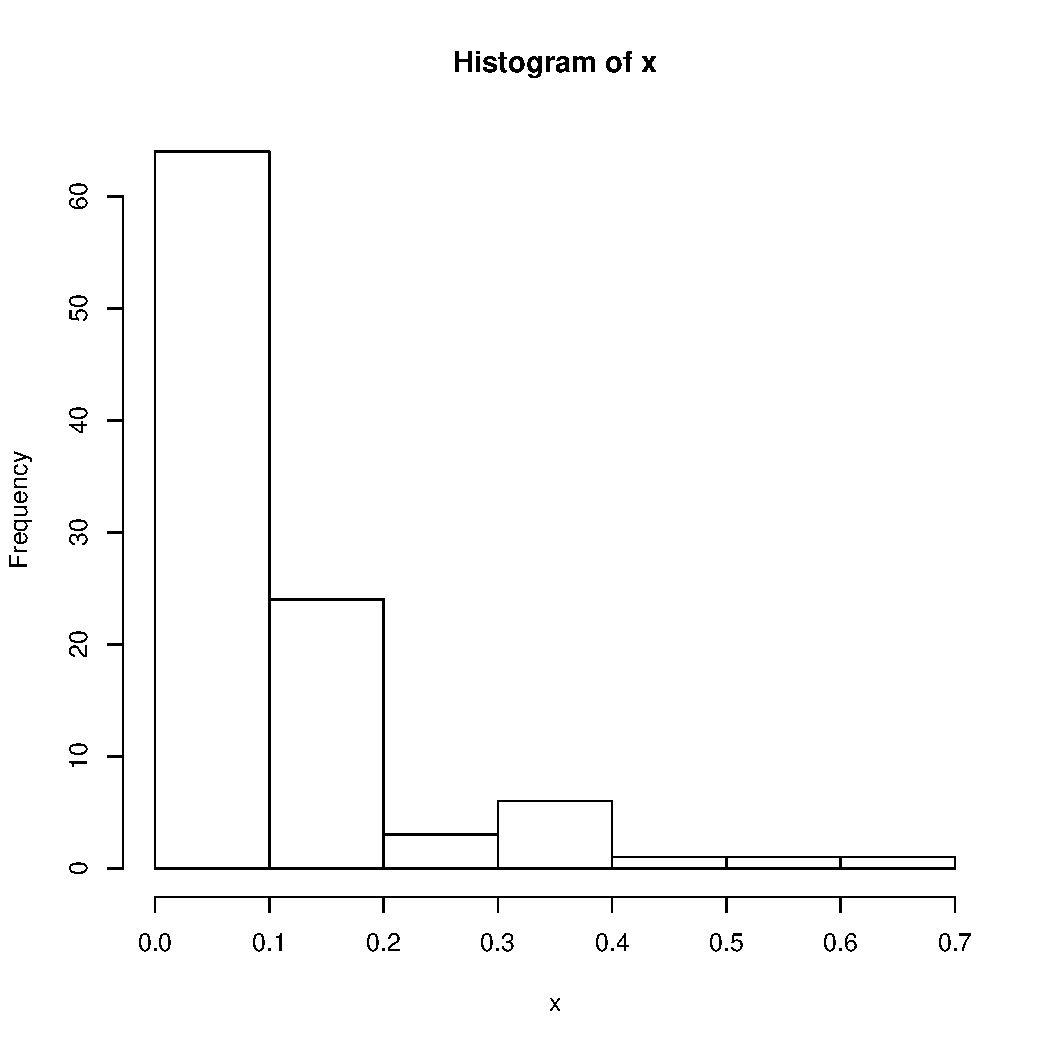
\includegraphics[width=.8\textwidth]{Histogram_Sample.pdf}
      \end{figure}
    \end{column}
  \end{columns}
\end{frame}

\begin{frame}[fragile]{Колмогоров--Смирнов тест}{Пример во R}
  Од обликот на хистограмот, претпоставуваме дека податоците имаат
  експоненцијална распределба.  Параметарот \(\lambda\) ќе го оцениме преку
  \(\bar{X}\).
\begin{minted}{R}
> 1 / mean(x)
[1] 9.54112
> ks.test(x, "pexp", rate=9.5)

	One-sample Kolmogorov-Smirnov test

data:  x
D = 0.063706, p-value = 0.8118
alternative hypothesis: two-sided
\end{minted}
  Ова е силен показател дека нултата хипотеза е точна, т.е.\ дека
  \(X \sim \mathcal{E}(\num{9.5})\).
\end{frame}

\section{Линеарна регресија}

\begin{frame}{Проста линеарна регресија}{Вовед}
  \begin{itemize}
  \item Претпоставуваме модел
    \[
      Y = \beta_0 + \beta_1 X + \epsilon\text{,}
    \]
    каде \(\beta_0\) и \(\beta_1\) се коефициенти, а
    \(\epsilon \sim \mathcal{N}(0, \sigma^2)\) е случајна компонента.
  \item Дадени оценки \(\hat{\beta}_0\) и \(\hat{\beta}_1\), вршиме предвидувања
    \[
      \hat{y} = \hat{\beta}_0 + \hat{\beta}_1 x\text{,}
    \]
    каде \(\hat{y}\) означува предвидување на \(Y\) за дадено \(X = x\).
  \end{itemize}
\end{frame}

\begin{frame}[fragile]{Проста линеарна регресија}{Пример во R}
  R ја содржи функцијата \mintinline{R}{lm} која служи за креирање линеарни
  модели.  Таа како аргумент прима објект од тип формула кој кажува кои се
  зависни а кои независни променливи.
\begin{minted}{R}
> advertisting <- read.csv("data/advertisting.csv",
+                          row.names=1)
\end{minted}
  Овие податоци даваат информација за успешност (sales) на различни методи за
  рекламирање (TV, Radio, и Newspaper).

  Сега, сакаме да провериме дали постои (линеарна) врска помеѓу продажбата и
  рекламирањето на ТВ.
\end{frame}

\begin{frame}[fragile]{Проста линеарна регресија}{Пример во R}
\begin{minted}[mathescape]{R}
> model <- lm(Sales ~ TV, data=advertisting)
> model.coefficients  # $\hat{y} = \num{7.03259355} + \num{0.04753664} x$.
(Intercept)          TV
 7.03259355  0.04753664
\end{minted}
  \begin{figure}
    \centering
    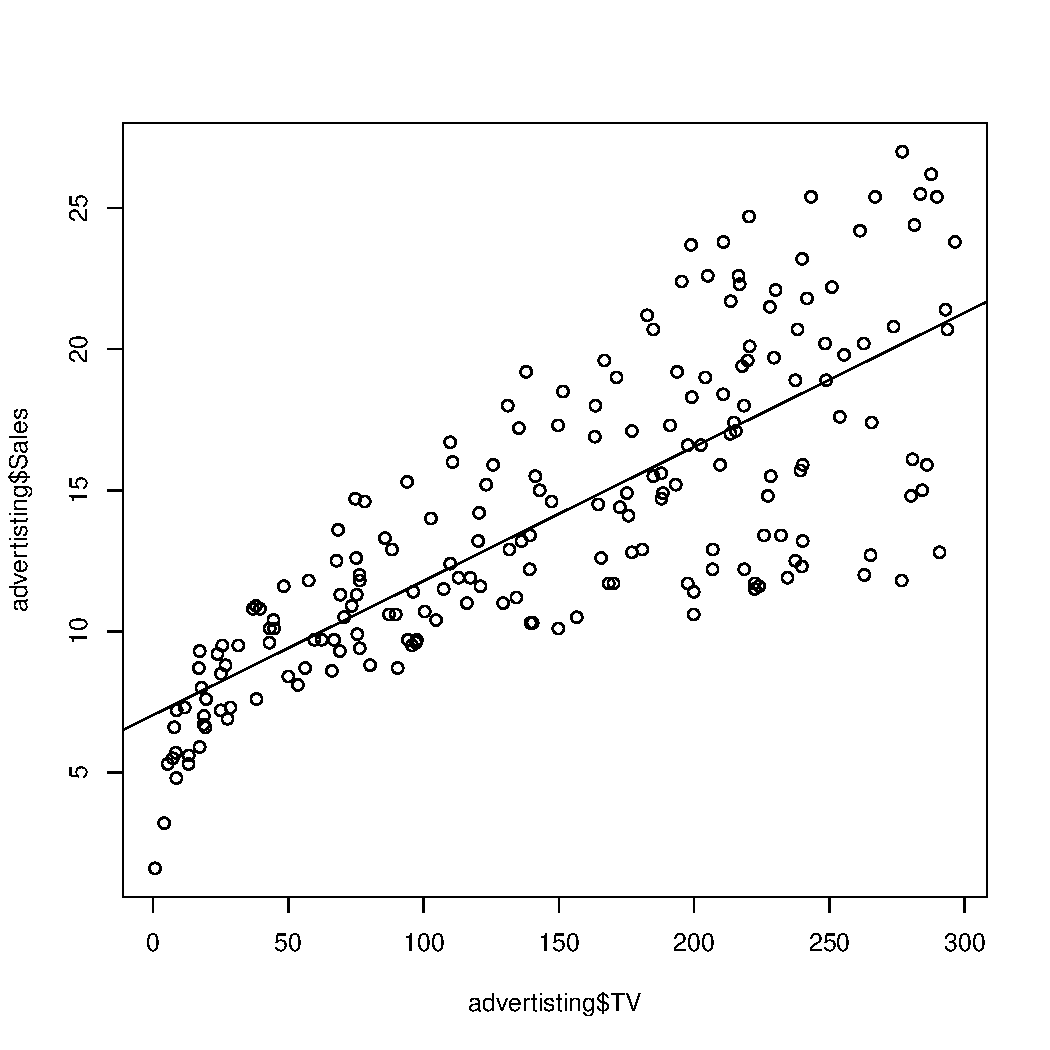
\includegraphics[width=.45\textwidth]{Plot_Simple_Regression.pdf}
  \end{figure}
\end{frame}

\begin{frame}[fragile]{Проста линеарна регресија}{Тестирање за значајност на
    \(\beta_1\)}
  Доколку сакаме да знаеме дали линеарната врска е значајна, т.е.\ дали
  \(\beta_1 \ne 0\), ја користиме статистикта
  \[
    T = \frac{\hat{\beta}_1}{\sigma / \sqrt{\sum\nolimits_{i = 1}^{n} (x_i -
        \bar{x})^2}} \sim t_{n - 2}\text{.}
  \]
  Во R оваа, како и други статистики поврзани со моделот, можеме да ги
  разгледаме со функцијата \mintinline{R}{summary}.
\begin{minted}{R}
> summary(model)$coefficients
              Estimate  Std. Error  t value    Pr(>|t|)
(Intercept) 7.03259355 0.457842940 15.36028 1.40630e-35
TV          0.04753664 0.002690607 17.66763 1.46739e-42
\end{minted}
  Од овде заклучуваме дека и двата коефициенти се значајни.
\end{frame}

\begin{frame}[fragile]{Линеарна регресија}
  \begin{itemize}
  \item Обопштување на претходниот случај.
  \item Претпоставуваме модел
    \[
      Y = \beta_0 + \beta_1 X_1 + \beta_2 X_2 + \ldots + \beta_p X_p +
      \epsilon\text{,}
    \]
    каде \(\beta_i\) се коефициенти, а
    \(\epsilon \sim \mathcal{N}(0, \sigma^2)\) е случајна компонента.
  \item Процеудрата во R е иста, со тоа што на десната страна на формулата
    додаваме повеќе независни променливи.
\begin{minted}{R}
> model <- lm(formula = Sales ~ TV + Radio + Newspaper,
+             data = advertisting)
> summary(model)$coefficients['Newspaper', 'Pr(>|t|)']
[1] 0.8599151
\end{minted}
    Гледаме дека продажбата не зависи од рекламирањето во весник (коефициентот
    пред Newspaper е \num{0}).
  \end{itemize}
\end{frame}

\end{document}

%%% Local Variables:
%%% mode: latex
%%% fill-column: 80
%%% TeX-command-extra-options: "-shell-escape"
%%% TeX-master: t
%%% End:
